\documentclass{suesmmthesis}
\facultyname{学院名称}
\subjectname{专业名称}
\classname{班级名称}
\teamnumber{M123456789}
\teammemberA{队员A}
\teammemberB{队员B}
\teammemberC{队员C}
\suesmmtitle{第十四届研究生数学建模竞赛}
\contenttitle{数学建模竞赛论文的使用方法}
\keywords{使用方法,latex}
\begin{document}
    \makecover
    \begin{abstract}
        请至少使用 \TeX Live 2019,XeLaTeX 编译,请选用支持 UTF­-8 编码的编辑器。

		使用者需要有一定的 \LaTeX{} 的使用经验,因此本文没有介绍基础使用,至少要会使用常用宏包的一些功能,比如参考文献,数学公式,图片使用,列表环境等等。模板已经添加了常用的宏包,无需用户再额外添加。

		本模板
		\begin{itemize}
			\item 本模板参考上海工程技术大学数学建模竞赛论文Word模板修改,方便学校同学使用;
			\item 图片应放在 \lstinline|figure| 文件夹中;
			\item 加载了 \lstinline|cleveref| 宏包,使用方法:\lstinline|\cref{label}|。
		\end{itemize}
	
		欢迎下载使用本模板,本模板代码地址为\href{https://github.com/MobtgZhang/sues-mm}{Github地址},并且此代码已经部署到\href{https://www.overleaf.com/read/mynpkfvwqjnm}{Overleaf}上,可以提供给大家正常使用。同时也欢迎大家到我的GitHub上提交issue,以方便模板的更新。
    \end{abstract}
    \tableofcontents
    \newpage
    \section{问题重述}
    问题重述不是照抄原题!

    数学建模比赛论文是要我们解决一道给定的问题,所以正文部分 一般应从问题重述开始,一般确定选题后就可以开始写这一部分了。

    这部分的内容是将原问题进行整理,将问题背景和题目分开陈述即可,所以基本没啥难度。

    本部分的目的是要吸引读者读下去,所以文字不可冗长,内容选择不要过于分散、琐碎,措辞要精练。

    问题重述应该在仔细理解了问题的基础上,用自己的语言重新将问题描述一遍。语言需要简明扼要,没有必要像原题一样面面俱到。
    \section{模型假设}
    根据全国组委会确定的评阅原则,基本假设的合理性很重要。

    \begin{enumerate}[label=(\arabic*)]
        \item 根据题目中条件作出假设;
        \item 根据题目中要求作出假设。
    \end{enumerate}
    
    关键性假设不能缺;假设要切合题意
    \section{符号说明}
    下面是一个参考的列表,可以作为符号说明。
    \begin{center}
		\begin{tabular}{p{0.24\textwidth}<{\centering}p{0.68\textwidth}<{\centering}}
			\toprule[1.5pt]
            符号 & 符号说明\\
            \midrule[0.75pt]
			$\delta$ & 赤纬角\\
			$\beta$ & 经度\\
			$\alpha$ & 纬度\\
			$r$ & 地球半径\\
			$\gamma$ & 太阳光与杆所成的夹角\\
			$l$ & 杆的长度\\
			$l_{y}$ & 杆的影子长度\\
			$\vec{x}_{1},\vec{y}_{1},\vec{z}_{1}$ & 由杆的位置所生成的切平面的正交基\\
			$\vec{\hat{x}}_{1},\vec{\hat{y}}_{1},\vec{\hat{z}}_{1}$ & 由杆的位置所生成的切平面的单位正交基\\
			$\theta$ & 影子与北方的夹角\\
			$l_{y}(i)$ & 编号为 $i$ 的数据对应的影子长度\\
			$\theta_{i}$ & 编号为 $i$ 的数据对应的影子角度\\
			\bottomrule[1.5pt]
		\end{tabular}
	\end{center}

    \section{模型的建立与求解}
    \subsection{问题一求解}
    效果见\cref{fig:exmaple1}。
	\begin{figure}[htbp]
		\centering
		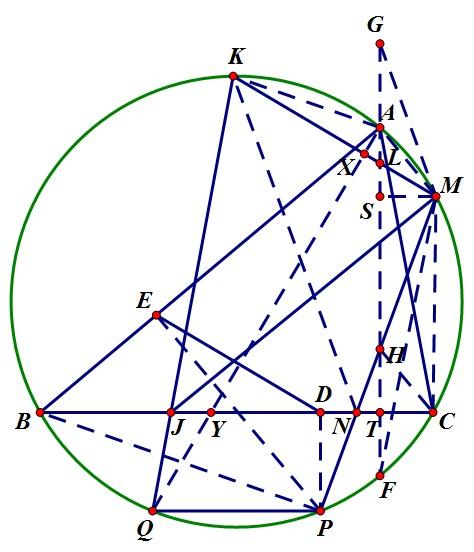
\includegraphics[width=0.3\textwidth]{example1.jpg}
		\caption{这里是一个示例样图作参考}
        \label{fig:exmaple1}
	\end{figure}
    \subsection{问题二求解}
    在遇到规划问题是最先且重要的步骤是:

    \begin{itemize}
        \item 确定决策变量;
        \item 确定建立线性模型前先使用SPSS或者spsspro对决策变量进行拟合,根据拟合效果选择;
        \item 建立目标函数;
        \item 列出约束条件;
    \end{itemize}

    线性规划的目标函数可以是求解最大值,也可以是求解最小值,约束条件的额不等号可以是小于号也可以是大于号。为了避免这种形式多样性带来的不便,MATLAB当中规定线性规划的标准形式为
    \begin{equation}
        \min\limits_{x}{c^{T}x}
    \end{equation}
    \begin{equation}
        \text{s.t.}\begin{cases}
            Ax\leq{b}\\
            Aeq\cdot{x}=beq\\
            lb\leq{x}\leq{ub}
        \end{cases}
    \end{equation}

    其中$c$和$x$均为$n$维向量,$A$、$Aeq$为适当维数的矩阵,$b$、$beq$为适当维数的列向量。
    \subsection{问题三求解}
    线性规划,适用的问题有:
    \begin{itemize}
        \item 运输问题
        \item 指派问题
        \item 对偶理论与灵敏度分析
        \item 投资的收益和风险
    \end{itemize}
    \section{模型评价与推广}
    \subsection{模型优点}
    本模型相对于已经存在的模型,具有以下的一些优点
    \begin{itemize}
        \item 具有较好的稳定性,模型的健壮性较强;
        \item 具有较好的鲁棒性,特别是在加入干扰因素之后,依旧模型预测结果保持较好。
    \end{itemize}
    \subsection{模型缺点}
    本模型但是还存在以下很多缺点:
    \begin{enumerate}[label=\arabic*)]
        \item 模型还有结构不合理的地方,不能够保证参数的平滑性;
        \item 模型通用性不太好,只能适用在特定的领域当中发挥作用。
    \end{enumerate}
    \section{结论}
    我们参考了文献\cite{LiuChangping2011},文献\cite{ChenKai2014},通过建模讨论发现这些问题,然后我们在此基础之上改进了很多较好的方法,最后得到了最新的结论。
    \newpage
    % 参考文献
    %设置参考文献风格,参照使用 https://github.com/Haixing-Hu/GBT7714-2005-BibTeX-Style
    \bibliographystyle{gbt7714-2005}
    \nocite{*}
    \bibliography{refers}
    \newpage
    \appendix
    \section{Matlab参考代码}
\begin{lstlisting}[language=matlab,caption={The matlab Source code of Algorithm}]
kk=2;[mdd,ndd]=size(dd);
while ~isempty(V)
[tmpd,j]=min(W(i,V));tmpj=V(j);
for k=2:ndd
[tmp1,jj]=min(dd(1,k)+W(dd(2,k),V));
tmp2=V(jj);tt(k-1,:)=[tmp1,tmp2,jj];
end
tmp=[tmpd,tmpj,j;tt];[tmp3,tmp4]=min(tmp(:,1));
if tmp3==tmpd, ss(1:2,kk)=[i;tmp(tmp4,2)];
else,tmp5=find(ss(:,tmp4)~=0);tmp6=length(tmp5);
if dd(2,tmp4)==ss(tmp6,tmp4)
ss(1:tmp6+1,kk)=[ss(tmp5,tmp4);tmp(tmp4,2)];
else, ss(1:3,kk)=[i;dd(2,tmp4);tmp(tmp4,2)];
end;end
dd=[dd,[tmp3;tmp(tmp4,2)]];V(tmp(tmp4,3))=[];
[mdd,ndd]=size(dd);kk=kk+1;
end; S=ss; D=dd(1,:);
\end{lstlisting}
    \section{Python参考代码}
\begin{lstlisting}[language=python,caption={The python Source code of Algorithm}]
#辗转相除
def divisor(n,m):
    d=1
    while d!=0:
            c=n/m   #商数
            d=n%m   #余数
            n=m     #替换除数
            m=d     #替换被除数
    return n

#判断大小
def judge(n,m):
    if n>m:
        re=divisor(n,m)
    else:
        re = divisor(m, n)
    return re

#主函数
s=judge(100,18)
print(s)
\end{lstlisting}
\end{document}

